\documentclass[12pt] {article}
\usepackage[top=1.75in, bottom=1.75in, left=1.75in, right=1.75in]{geometry}
\usepackage[pdftex]{hyperref}
\usepackage{graphicx}
\usepackage{float}
\hypersetup{
	pdfauthor={Phil Monroe and Kramer Straube},
	pdftitle={Face Detection on the GPU}}
	
\begin{document}

% Title
\centerline{\Large \bf Face Detection on the GPU}

% Author
\centerline{\bf Phil Monroe and Kramer Straube}

% Date
\centerline{Mar. 15, 2012}
\medskip

\begin{abstract}
In this paper, we implemented the beginnings of the Viola-Jones object detection method as it applies to faces. We also added a single feature classifier to detect the presence of glasses. To implement this on the GPU, we first find the integral image which is done serially because it is faster. Then, we cascade our identifiers and apply them using the integral image to minimize memory accesses. Finally, if any sub-windows pass all classifiers, it is concluded that the image contains a face. This simple implementation provides 97.3\% accuracy at detecting faces, 96\% accuracy at detecting glasses, a false positive rate of 76\% for faces and 21.1\% for faces and runs at a rate of 46 images scanned per second. We also evaluated a non-cascaded Viola-Jones implementation and found it to be slower. At the end, we discuss how the Viola-Jones algorithm can be manipulated to scale more efficiently to the GPU.
 
\end{abstract}

\section{Introduction}
In this paper, we will address the application of face detection on the GPU. We used the Viola-Jones Object Detection algorithm to detect faces. We also added a glasses identifier to make an attempt at detecting whether the faces detected had glasses or not. We tested our algorithm on a subset of the Caltech Web Faces database and a subset of the Caltech 101 image database to analyze how accurate our implementation was. Finally, we discuss the pros and cons of the implementation as well as some notable aspects of our specific implementation.


%Do we need to mention how we make sub-windows? (how many / image)
\section{Viola-Jones Object Detection}
Viola-Jones object detection focuses on using simple identifiers to determine whether the object exists in the image or not. The algorithm also performs object localization if sufficiently many identifiers are used. We used this algorithm to determine the presence (or lack thereof) of a face in an input image. The algorithm splits the image into numerous \emph{sub-windows} or small regions of the image upon which detection is applied. Sub-windows help the algorithm to distinguish between small and large faces within an image. The sub-window size is computed in this implementation by taking the smaller image dimension (rows or columns) and dividing by four.


% Integral Image -----------------------------------------------------------------
\subsection{Integral Image}
To speed up computation of the identifiers, the Viola-Jones algorithm pre-computes the integral image. The integral image defines each pixel as the sum of all pixels that are both above and to the left of it. We explored both the standard serial implementation of computing the integral image from OpenCV as well as a parallel implementation.

The parallel implementation first performs a scan operation on the columns to create a sum for each pixel location of all the pixels above it. Then, the algorithm does a scan operation on the rows to add up all of the column sums for each pixel to the left of it. This calculates the sum of all of the pixels above and to the left of the current pixel.


% Cascade of Classifiers -----------------------------------------------------------------
\subsection{Cascade of Classifiers}
The classifiers are simple rectangular identifiers to determine different features of the face. To compute whether the classifier accepts that the given sub-window has a face, the algorithm subtracts the "black" area from the "white" area of the classifier. Figure 1 shows the classifiers we used for face detection. In the Viola-Jones paper, they use two hundred of these kinds of classifiers but we use a small subset of four classifiers because we are interested in how this algorithm applies to the GPU instead of the actual results. Four was sufficient to see the difficulties with implementing this algorithm on the GPU.

The other portion of Viola-Jones face detection was the use of a classifier \emph{cascade}. This means that the output of one classifier (which contains the list of sub-windows that may have a face) is the input for the next classifier. So if any classifier rejects a sub-window, the algorithm rejects the sub-window. If all of the classifiers accept a sub-window, then the algorithm says that there is a face at that sub-window. The alternative to the cascade approach is to apply all of the classifiers to every sub-window and define some number of acceptances that each sub-window needs to determine that there is a face there. We implemented both of these approaches to analyze which would be more efficient on the GPU.
\begin{figure}[h!]
	\centering
		
\includegraphics[width=60mm]{classifiers.pdf}
		\caption{The set of identifiers used in our implementation of Viola-Jones}
\end{figure}


% Glasses Classifier -----------------------------------------------------------------
\subsection{Glasses Classifier}
To extend the Viola-Jones face detection algorithm, we added a glasses classifier at the end of the classifier cascade to detect whether the face had glasses or not. Figure 2 shows the glasses classifier that we designed. The idea behind this classifier is that it will pick up on the portions of the frame that are on top of skin. Thus, the darker frame will be subtracted from the lighter skin areas on both the bridge of the glasses and the portion that goes, from the front, back to the ears.
\begin{figure}[h!]
	\centering
		
\includegraphics[width=30mm]{glasses_identifier.pdf}
		\caption{The glasses classifier that we implemented}
\end{figure}


% Results -----------------------------------------------------------------
\section{Results}
We ran the cascaded algorithm with three different datasets: faces, non-faces, and faces with glasses. The cascaded algorithm running on the faces dataset with 50 pictures produced a result of 49 faces detected and zero glasses detected. The same algorithm running with the non-face dataset with 50 pictures resulted in 38 faces detected and 8 glasses detected. The face detector ran on the glasses dataset with 25 pictures and found 24 face, 20 of which had glasses. Overall, the face detector has weak results with an accuracy of 97.3\% but a false positive rate of 76\%. The glasses classifier did well with an accuracy of 83.3\% and a false positive rate of 21.1\%. The entire cascaded face detection algorithm ran in 0.020334 seconds. The non-cascaded algorithm ran 65\% slower at 0.033715 seconds. The glasses classifier ran in 0.004104 seconds. These timings are not absolute because it depends on the image and how the cascade can eliminate sub-windows early (reducing work for later stages). In a simple extrapolation of our timing results, we took the glasses classifier and assumed that all later classifiers in a 200-classifier Viola-Jones parallel implentation would complete in that much time. The result was that it would take 824.718 ms to complete. This result is pessimistic because the cascade of classifiers would cause fewer and fewer sub-windows to be evaluated. All of our timing and accuracy results are found in Tables 1 and 2. Figure 4 shows a sample run of our implementation on the image given in Figure 3. In this image, the brighter spots lasted further through the cascade.

\begin{center}
	\begin{table}[h!]
		\caption{Face Detection Results}
		\centering
		\medskip

		\scalebox{0.76}{
			\begin{tabular}{ | l | c | c | c | p{4cm} |}

				\hline
				Dataset & Faces Found & Glasses Found & Total Files & Comment 	\\ \hline
				Faces 					& 49 	& 0 	& 50 	& 98\% Accuracy			\\ \hline
				Non-Faces 				& 38 	& 8 	& 50	& 76\% False Positive	\\ \hline
				Faces with Glasses 	& 24 	& 20 	& 25	& 96\% Face Accuracy
				\newline 80\% Glasses Accuracy	\\ \hline

			\end{tabular}
		}
	\end{table}

	\begin{table}[h!]
		\centering
		\caption{Face Detection Performance}
		\medskip

		\scalebox{0.76}{
			\begin{tabular}{ | l | c | l |}

				\hline
				Operation	 						& Time (ms) 			& Comment 	\\ \hline
				Serial Integral Image			& 1.277					&				\\ \hline
				Parallel Integral Image			& 9.329 					& 	Much slower than serial\\ \hline
				Parallel Face Detection 		& 20.334 				&				\\ \hline
				Glasses Detection 				& 4.104 					&				\\ \hline
				Brute Force Face Detection 	& 33.715 				&				\\ \hline
				Extrapolated 200 Feature Cascade in Parallel  & 824.718    & \\ \hline
			\end{tabular}
		}
	\end{table}

\end{center}

\begin{figure}[h!]
	\centering
		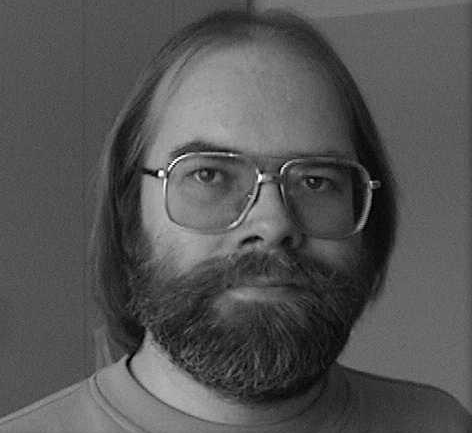
\includegraphics[width=80mm]{face.png}
		\caption{The input for the sample run}
\end{figure}

\begin{figure}[h!]
	\centering
		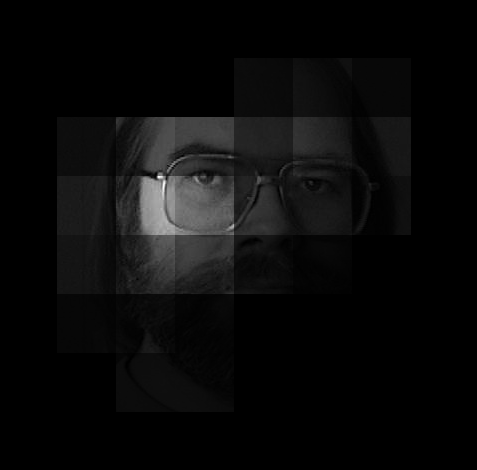
\includegraphics[width=80mm]{heatmap.png}
		\caption{The output heatmap for the example run}
\end{figure}


% Discussion -----------------------------------------------------------------
\section{Discussion}
This implementation of the Viola-Jones algorithm performed fairly well with the only real downside being the 76\% false positive rate. To fix this, more classifiers can be implemented to describe a face much better than the four simple classifiers used. Sources show that using up to 200 classifiers can weed out the false positives. That being said, our detector did show 97.3\% accuracy in finding faces and can be run at a rate around 46 images per second, which is fast enough for real time classification. The image rate will drop as the number of classifiers is increased, but sources show that the algorithm can achieve faster than 25 images per second on newer GPUs.

A fault was found in our implementation during while tuning the classifiers that is worth noting. The third identifier used was providing negative fit values which makes it interesting to threshold. To combat this, the absolute value of the fit value is used to be thresholded. This is bad since it makes the third and fourth classifiers effectively the same. The classifier was left in due to time constraints and to help show timing results. 

It is interesting to point out that the parallel computation of the integral image performed much slower than computing the image on the CPU. This is since computing the integral image is very simple and iterative, which makes excellent use of the CPU's caches. On the GPU, the bottleneck becomes the lack of mathematical computation compared to the number of memory accesses. This is compounded when memory coalescing is taken into effect. Depending on how the image is stored in memory, on of the passes will coalesce and the other will not, causing the GPU implementation to slow down even more.

It is also worth mentioning the comparison of the cascading classifier method vs. the brute force computation of all classifiers. By cascading classifiers, full GPU occupancy can be achieved by increasing the number and size of sub-windows as well as classifier scales being run concurrently. As sub-windows start to be eliminated, the GPU starts wasting cycles by not filling all cores with work to do. This reduction in sub-windows is a big win for the serial implementation, however more computation could be exploited using a GPU. The brute force method of computing all classifiers in parallel was considered to improve maximum occupancy. While the brute force method did take longer than the cascading approach, it provides more detailed results about what each sub-window contains which can be used in smarter, tournament style detectors. 

% Conclusion -----------------------------------------------------------------
\section{Conclusion}
This project provided an implementation of the Viola-Jones face detection on the GPU with the added functionality of glasses detection. This simplified version was able to detect faces with an accuracy of 97.3\% and glasses at 96\% accuracy. The drawback of the simple implementation is the rather large 76\% false positive rate. This project did bring about many interesting discoveries about the detection algorithm, such as the benefit of serial integral image computation and the brute force parallel classifier computation.

% References -----------------------------------------------------------------
\footnotesize
\section{References}

\begin{itemize}
	\item Viola, Jones: {\it Rapid Object Detection using a Boosted Cascade of Simple Feature} - \url {http://bit.ly/pgwskh}
	\item Viola, Jones: {\it Robust Real-time Object Detection} - \url {http://bit.ly/genUvI}
	\item Hefenbrock, Oberg, et. al. {\it Accelerating Viola-Jones Face Detection to FPGA-Level using GPUs} - \url {http://bit.ly/yRxbc4}
	\item Patil: {\it Face Detection on GPU} - \url {https://sites.google.com/site/facedetectionongpu/}
	\item Obukhov: {\it Face Detection with CUDA} - \url {http://www.slideshare.net/NVIDIA/1071-gtc09}
	\item Thrust CUDA Algorithm Library - \url {http://code.google.com/p/thrust}
\end{itemize}

% Source Code -----------------------------------------------------------------
\section{Source Code and Project Files}

\hspace*{1.5em}The website containing all project files can be found at:
\newline \url {http://phil-monroe.github.com/EEC-277---GPU-Face-Detect/}
\vspace{5 mm}

The source code is hosted on GitHub at:
\newline \url {https://github.com/phil-monroe/EEC-277---GPU-Face-Detect}



\end{document}

